%% formulation.tex
%% Technical reference document: Spacecraft CA SDec-POMDP Formulation
%% Compile: pdflatex formulation.tex

\documentclass[11pt]{article}
\usepackage[margin=1in]{geometry}
\usepackage{amsmath, amssymb, amsthm}
\usepackage{booktabs}
\usepackage{hyperref}
\usepackage{xcolor}
\usepackage{enumitem}
\usepackage{titlesec}
\usepackage{graphicx}

\definecolor{todo}{RGB}{200,50,50}
\newcommand{\TODO}[1]{\textcolor{todo}{\textbf{[TODO: #1]}}}
\newcommand{\norm}[1]{\left\lVert#1\right\rVert}

\title{\textbf{Semi-Decentralized Multi-Spacecraft Collision Avoidance\\
under Communication Constraints}\\[0.5em]
\large POMDP Formulation \& System Architecture}
\author{Grace Ra Kim, Mahdi Al-Husseini, Duncan Eddy, Mykel J.\ Kochenderfer}
\date{\today}

\begin{document}
\maketitle
\tableofcontents
\bigskip

% =============================================================================
\section{Problem Overview}
% =============================================================================

Two active spacecraft are on a conjunction trajectory in LEO. Each spacecraft is
controlled by a separate ground operator who receives state updates and conjunction
data only during intermittent ground-station contact windows. Operators must plan
impulsive maneuvers under partial observability and limited coordination.

We model this as a \textbf{Semi-Decentralized POMDP (SDec-POMDP)} solved with
Recursive Small-Step Semi-Decentralized A* (RS-SDA*). Ground-station contact
windows define synchronization triggers --- the moments when agents may share
beliefs and take joint actions.

\subsection{Key Design Philosophy}

The state space is built around \textbf{predicted miss distance at TCA} rather
than raw RTN position. This choice is motivated by three factors:
\begin{enumerate}
  \item Miss distance is what CDMs report and what operators reason about.
  \item The collision reward depends directly on miss distance at TCA --- using
        it as state makes the reward trivially correct.
  \item It collapses a 6D relative state into a scalar, keeping the discrete
        model tractable.
\end{enumerate}

Orbital propagation (Brahe) is used \emph{offline only} to build the transition
matrix. RS-SDA* operates entirely on precomputed $T$, $O$, $R$ arrays.

\subsection*{Note on Communication Variables in State}

The abstract describes a state space that includes communication variables
(ground-station visibility, most recent comms status). In our implementation,
these are \textbf{not} included as state variables. Instead, communication
structure is encoded entirely via the \texttt{sync\_states} list passed to
\texttt{SDecPOMDPModel} --- the set of states at which agents synchronize.

This is the standard pattern across all RS-SDA* benchmarks (Mars rovers,
Tiger, Labyrinth): the physical state is the domain state only, and the
trigger list encodes when coordination occurs. For our domain, ground contact
windows are deterministic and known upfront, so the sync trigger list captures
the communication structure completely without redundancy. Comms variables in
state would add complexity with no expressive benefit given a fixed, known
contact schedule.

% =============================================================================
\section{Conjunction Geometry}
% =============================================================================

\subsection{Geometry Type: Radial-Miss}

We use a \textbf{radial-miss} conjunction geometry. In the RTN (Radial-Transverse-Normal)
frame centered on SC1:

\begin{itemize}
  \item \textbf{R (Radial)}: points outward from Earth's center through SC1.
        This is the \emph{collision axis} --- SC2 is offset in R at TCA.
  \item \textbf{T (Transverse / Along-track)}: points in the direction of orbital
        motion. SC2 approaches SC1 from behind (negative T), closing at
        $v_\text{rel} \approx 15$\,m/s.
  \item \textbf{N (Normal / Cross-track)}: perpendicular to the orbital plane.
        $\delta N \approx 0$ throughout --- negligible cross-track motion.
\end{itemize}

At TCA, the geometry is:
\begin{equation}
  \delta \mathbf{r}_\text{RTN}^\text{TCA} =
    \begin{bmatrix} d_\text{miss} \\ 0 \\ 0 \end{bmatrix}, \quad
  \delta \mathbf{v}_\text{RTN}^\text{TCA} =
    \begin{bmatrix} 0 \\ -v_\text{rel} \\ 0 \end{bmatrix}
\end{equation}
where $d_\text{miss}$ is the miss distance (radial separation at closest approach)
and $v_\text{rel} = 15$\,m/s is the along-track closing speed.

\begin{figure}[h]
\centering
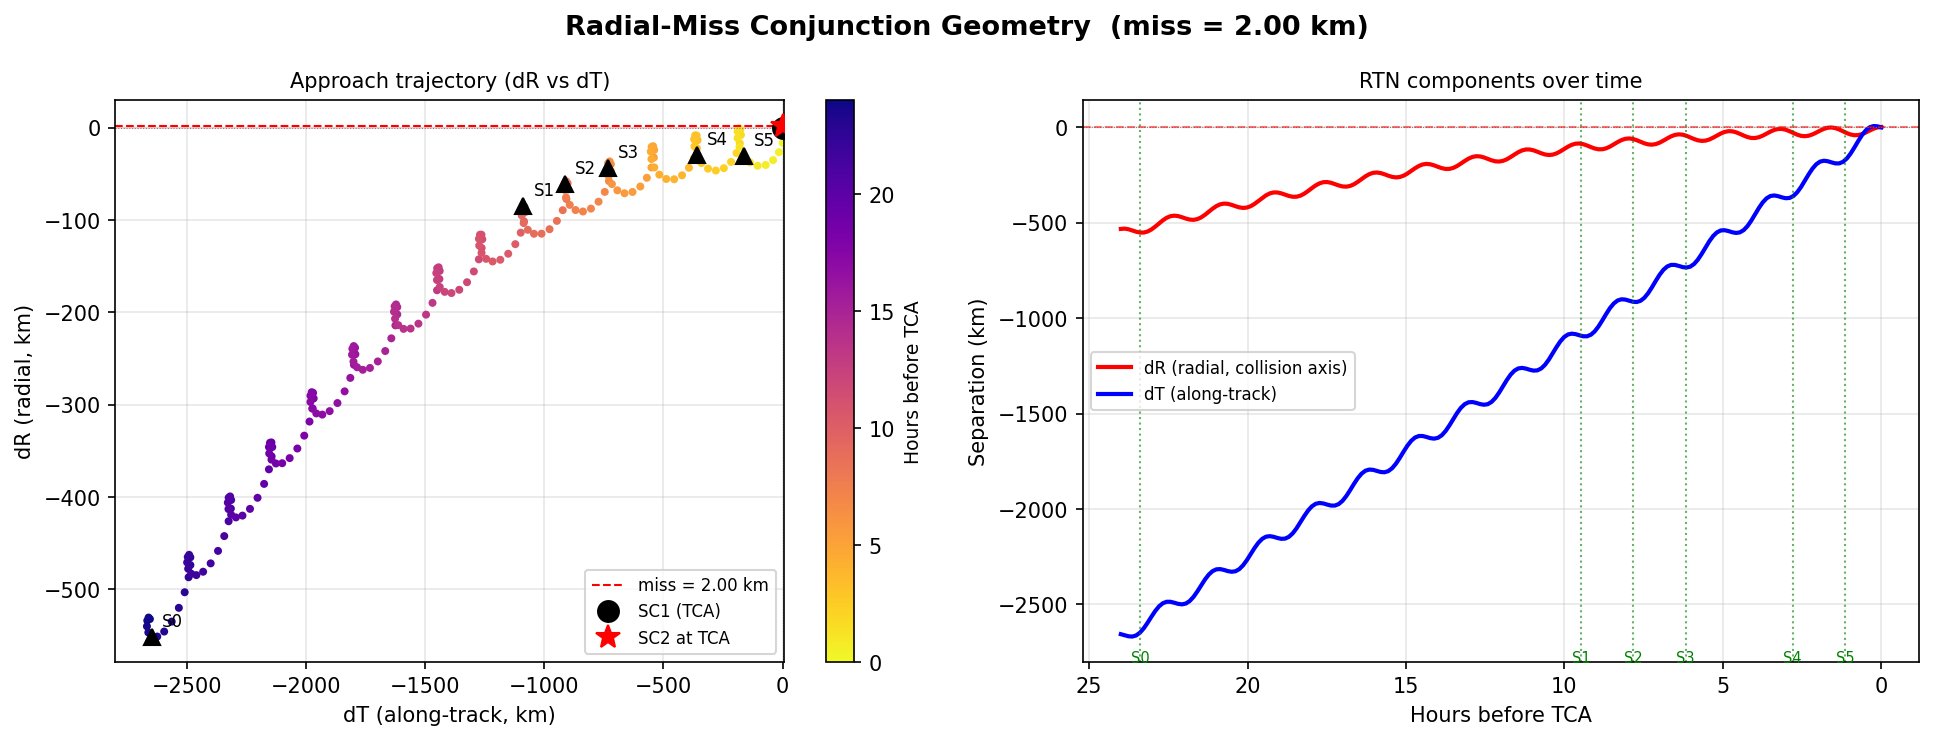
\includegraphics[width=0.7\textwidth]{../figures/conjunction_geometry.png}
\caption{Radial-miss conjunction geometry in the RTN frame at TCA.
SC2 is offset from SC1 in the radial direction by the miss distance.
SC2 approaches from the along-track direction (negative T), with relative
velocity entirely in T at TCA.}
\end{figure}

\noindent\textbf{Why radial-miss (not crossing):} A crossing conjunction has
the miss distance in the N (cross-track) direction. Discretizing N into bins
while keeping the RTN state tractable collapses the collision zone to a
single bin that is never reached from nominal trajectories. Radial-miss places
the collision axis in R, which is directly captured by the POMDP state
(miss distance bin), and along-track maneuvers ($\Delta v_T$) shift the
radial offset at TCA in a predictable, bin-differentiating way.

\subsection{Orbit and Scenario Parameters}

\begin{itemize}
  \item \textbf{Orbit}: 550\,km circular, 55$^\circ$ inclination
  \item \textbf{Planning horizon}: 24\,h before TCA
  \item \textbf{Relative speed at TCA}: $v_\text{rel} = 15$\,m/s (along-track)
  \item \textbf{Maneuver magnitude}: $\Delta v = 0.5$\,m/s (configurable;
        produces good bin differentiation at all planning horizons)
\end{itemize}

\subsection{Representative State for Matrix Generation}

Since the POMDP state is a scalar miss distance bin, each state must be mapped
to a representative 6D relative state for Brahe propagation. We use
\textbf{back-propagation from TCA}: SC2 is placed at the target miss distance at
TCA, then Brahe-propagated backward to the stage epoch.

\begin{enumerate}
  \item Place SC2 at TCA with RTN relative state:
    \begin{equation}
      \delta \mathbf{r}_\text{RTN}^\text{TCA} = [d_\text{miss},\; 0,\; 0]^\top, \quad
      \delta \mathbf{v}_\text{RTN}^\text{TCA} = [0,\; -v_\text{rel},\; 0]^\top
    \end{equation}
  \item Back-propagate SC2 from $\tau_\text{TCA}$ to $\tau_k$ (stage epoch) using Brahe.
  \item Forward-propagate from $\tau_k$ to $\tau_\text{TCA}$ (round-trip check) ---
        miss distance is recovered to $< 1$\,m accuracy across all stages and all bins.
\end{enumerate}

\noindent\textbf{Why back-propagation:} Placing SC2 at a radial offset at the
\emph{stage} epoch does not produce the target miss distance at TCA --- the radial
offset evolves under Keplerian dynamics and can differ by thousands of km after
24\,h of propagation. Back-propagation from TCA guarantees the representative
state has exactly the intended miss distance, independent of the planning stage.

% =============================================================================
\section{SDec-POMDP Formulation}
% =============================================================================

\subsection{State Space}

The global state at decision epoch $k$ is:
\begin{equation}
  s = (d_\text{miss},\; k)
\end{equation}
where $d_\text{miss}$ is the predicted miss distance at TCA (meters), discretized
into $N_d$ bins, and $k \in \{0, \ldots, H-1\}$ is the planning stage index.

\begin{table}[h]
\centering
\caption{Miss distance discretization}
\begin{tabular}{clc}
\toprule
Bin & Range & Interpretation \\
\midrule
0 & $[0,\; 1)$\,km   & Collision zone \\
1 & $[1,\; 5)$\,km   & High risk \\
2 & $[5,\; 20)$\,km  & Moderate risk \\
3 & $[20,\; 100)$\,km & Low risk \\
4 & $[100,\; 500)$\,km & Nominal approach \\
5 & $[500,\; \infty)$\,km & Safe \\
\bottomrule
\end{tabular}
\end{table}

\noindent Total states: $N_d \times H + 1 = 6 \times 6 + 1 = \mathbf{37}$
(including one sink state after the final stage).

\subsubsection*{Physical Interpretation of the State}

The state $(d_\text{miss}, k)$ is best understood as: \emph{at the current contact window
(stage $k$), what miss distance will the spacecraft have at TCA if no further maneuvers
are applied?}

\begin{itemize}
  \item \textbf{Stage 0 is $T{-}23.4$\,h} --- the earliest ground contact, 23.4 hours
        before TCA. The initial state is the predicted miss distance at this epoch.
  \item \textbf{WAIT invariant}: under no maneuver, the predicted miss distance at TCA
        does not change between stages (Keplerian dynamics are deterministic). A spacecraft
        in bin~0 at stage~0 will remain in bin~0 at TCA unless a burn is applied.
  \item \textbf{Starting in bin~0} means: at $T{-}23.4$\,h, the current conjunction
        assessment predicts a close approach of $< 1$\,km. This is a \emph{pre-identified}
        conjunction scenario, not a collision in progress --- the operators have 23\,h to act.
  \item \textbf{Burning at stage $k$} shifts the predicted miss distance for all future
        stages. A prograde or retrograde burn of $\Delta v_T = 0.5$\,m/s at stage~0
        moves the prediction from bin~0 ($\sim$0.5\,km) to bin~4 ($\sim$128\,km).
\end{itemize}

\noindent\textbf{Planning horizon and contact schedule}:
\begin{center}
\begin{tabular}{cll}
\toprule
Stage & Time before TCA & Interpretation \\
\midrule
0 & $T{-}23.4$\,h & Initial assessment; first opportunity to act \\
1 & $T{-}9.5$\,h  & Re-estimate miss from updated tracking \\
2 & $T{-}7.8$\,h  & Update \\
3 & $T{-}6.2$\,h  & Update \\
4 & $T{-}2.8$\,h  & Last practical burn window \\
5 & $T{-}1.1$\,h  & Final decision (small effect at late stage) \\
TCA & $T{-}0$\,h  & Closest approach; collision check; reward fires \\
\bottomrule
\end{tabular}
\end{center}

\subsection{Action Space}

Each agent independently selects an impulsive along-track maneuver:
\begin{equation}
  \mathcal{A}_i = \{\text{WAIT},\; +\Delta v_T,\; -\Delta v_T\}, \quad i \in \{1, 2\}
\end{equation}
Joint action space: $|\mathcal{A}| = 3^2 = 9$.

$\Delta v_T$ is a fixed magnitude burn (e.g.\ 1\,m/s for the discrete model;
operationally realistic values are 2--50\,mm/s). The burn is applied in the
along-track direction in ECI coordinates.

\subsection{Transition Model}

The transition $T(s' \mid s, a)$ is built offline using Brahe:

\begin{enumerate}
  \item From state $(d_\text{miss\_bin},\; k)$, reconstruct a representative
        RTN relative state at stage epoch $\tau_k$.
  \item Apply joint maneuver $a = (a_1, a_2)$ impulsively to SC1 and SC2.
  \item Propagate both spacecraft from $\tau_k$ to TCA using Brahe numerical
        integrator (two-body or with perturbations).
  \item Compute resulting miss distance $d'$ and bin it $\rightarrow$ next state
        $(d'_\text{bin},\; k+1)$.
  \item $T[a,\; s,\; s'] = 1$ (deterministic given bin-center representative state).
\end{enumerate}

The final stage ($k = H-1$) transitions to the sink state.

\noindent\textbf{Key property}: Because the state already encodes predicted miss
distance, the collision reward fires cleanly at the terminal transition without
any additional propagation.

\subsection{Observation Model}

Each agent $i$ receives a noisy estimate of the miss distance during ground
contact, modeled as Gaussian noise on the true miss distance:
\begin{equation}
  \tilde{d}_i \sim \mathcal{N}(d_\text{miss},\; \sigma_\text{obs}^2)
\end{equation}
with $\sigma_\text{obs} \approx 10$--50\,km (realistic CDM uncertainty).

Observations are discretized into the same $N_d$ bins. The observation
probability is:
\begin{equation}
  O(o \mid s, a) = \int_{\text{bin}_o} \mathcal{N}(\tilde{d};\; d_\text{miss}(s'),\; \sigma_\text{obs}^2)\; d\tilde{d}
\end{equation}
Joint observation: $o = (o_1, o_2)$, $|\mathcal{O}| = N_d^2 = 36$.

\textbf{Between ground contacts}: agents receive no observation update and act
on stale beliefs. This is the core source of partial observability in the model.

\subsection{Reward Function}

\begin{equation}
  R(s, a) = R_\text{collision}(s) + R_\text{maneuver}(a) + R_\text{comms}(a)
\end{equation}

\begin{itemize}
  \item \textbf{Collision penalty} (terminal, at last stage):
    \begin{equation}
      R_\text{collision}(s) =
      \begin{cases}
        -1000 & \text{if } d_\text{miss} < 1\,\text{km at TCA} \\
        0 & \text{otherwise}
      \end{cases}
    \end{equation}
  \item \textbf{Maneuver cost} (fuel / trajectory deviation proxy):
    \begin{equation}
      R_\text{maneuver}(a) = -10 \cdot \mathbf{1}[a_1 \neq \text{WAIT}]
                             -10 \cdot \mathbf{1}[a_2 \neq \text{WAIT}]
    \end{equation}
  \item \textbf{Communication cost} (Scenario 3 only):
    \begin{equation}
      R_\text{comms}(a) = -c_\text{sync} \cdot \mathbf{1}[\text{sync event at this stage}]
    \end{equation}
\end{itemize}

\TODO{Add trajectory deviation reward: penalize change in orbital elements
(e.g.\ semi-major axis deviation) accumulated over all maneuvers. This is the
``mission performance'' term from the abstract.}

\subsection{Decision Epochs and Planning Horizon}

Decision epochs are the midpoints of ground-station contact windows, computed
via Brahe's \texttt{location\_accesses()} visibility analysis
(\texttt{examples/test\_contacts.py}). For a 550\,km, 55$^\circ$ orbit over Goddard
Space Flight Center (lon $= -76.8^\circ$, lat $= 39.0^\circ$, 10$^\circ$ min
elevation), Brahe finds 6 SC1 passes over the 24\,h planning horizon. The nominal
6-contact schedule is:

\begin{table}[h]
\centering
\caption{Decision epochs for Scenario 1 (single GS)}
\begin{tabular}{ccc}
\toprule
Stage $k$ & Time before TCA & Epoch (UTC) \\
\midrule
0 & $-23.39$\,h & 2025-06-01 00:36 \\
1 & $-9.48$\,h  & 2025-06-01 14:31 \\
2 & $-7.83$\,h  & 2025-06-01 16:10 \\
3 & $-6.17$\,h  & 2025-06-01 17:49 \\
4 & $-2.80$\,h  & 2025-06-01 21:12 \\
5 & $-1.13$\,h  & 2025-06-01 22:52 \\
\bottomrule
\end{tabular}
\end{table}

\noindent\textbf{Note on the contact gap:} There is a $\sim$14\,h gap between Stage~0
($T{-}23.4$\,h) and Stage~1 ($T{-}9.5$\,h). This is a real orbital mechanics feature: at
55$^\circ$ inclination over a mid-latitude station, the spacecraft is below the
10$^\circ$ elevation horizon for roughly half its orbital period ($\sim$95\,min orbit).
Stages~1--5 cluster in the final 10\,h before TCA because the spacecraft makes several
successive passes during that window. This gives the policy many update opportunities
late in the horizon but a long ``blind'' period early on.

For Scenario~1, both spacecraft are in nearly identical orbits, so all 6 SC1 passes
are simultaneously visible to SC2 $\Rightarrow$ all 6 contact windows are joint
$\Rightarrow$ all 36 non-sink states are synchronization triggers.

\subsection{Synchronization Triggers}

Synchronization triggers are defined by ground-station contact windows.
A state is a sync trigger if both spacecraft have an active (or recent) contact
at that stage, enabling joint belief update and coordinated action.

\begin{itemize}
  \item \textbf{Scenario 1} (cooperative): all 6 stages are sync triggers
        $\rightarrow$ always centralized
  \item \textbf{Scenario 2} (asymmetric): SC2 follows a fixed policy; SC1
        syncs at stages 0--2 only
  \item \textbf{Scenario 3} (costly comms): all stages available but sync
        incurs $R_\text{comms}$ penalty; policy trades off coordination vs.\ cost
\end{itemize}

% =============================================================================
\section{System Architecture}
% =============================================================================

The system has three distinct components that run at different times:

\subsection{Component 1: Offline Matrix Builder (\texttt{spacecraft\_matrices.py})}

Runs once. Uses Brahe to precompute $T$, $O$, $R$ matrices and saves to
\texttt{.npz} cache.

\begin{verbatim}
For each (miss_bin, stage, joint_action):
  1. Reconstruct RTN relative state at stage epoch
  2. Apply maneuvers to SC1 and SC2
  3. Brahe-propagate both to TCA
  4. Measure miss distance -> bin -> T[a, s, s']
  5. Compute observation distribution -> O[a, s', o]
  6. Assign reward -> R[a, s]
Save T, O, R, init_b to spacecraft_matrices_cache.npz
\end{verbatim}

\subsection{Component 2: Policy Solver (\texttt{sdec\_spacecraft.py})}

Loads cached matrices, constructs \texttt{SDecPOMDPModel}, runs RS-SDA*.
Never calls Brahe. Outputs a policy $\pi(\text{belief}) \rightarrow$ action.

\begin{verbatim}
T, O, R, init_b = load_matrices()
model = SDecPOMDPModel(nagents=2, ...)
config = RSSDAConfig(maxh=6, algorithm="approximate", ...)
sdec = SDecPOMDP(model, config)
value, policy = sdec.multi_agent_astar(6)
\end{verbatim}

\subsection{Component 3: Simulator (\texttt{spacecraft\_simulator.py})}

Runs after policy is computed. Uses Brahe with real ECI states to evaluate
the policy in closed-loop simulation. Generates paper metrics.

\begin{verbatim}
Initialize true ECI states from conjunction generator
For each stage k:
  1. Propagate true states to stage epoch with Brahe
  2. Simulate noisy observation (miss distance estimate)
  3. Update belief
  4. If sync trigger: share beliefs, take joint action
  5. Else: each agent acts independently per policy
  6. Apply maneuver to true ECI states
At TCA: propagate to TCA, measure true miss distance
Record: miss distance, total dv, sync count, trajectory deviation
\end{verbatim}

\subsection{Data Flow Diagram}

\begin{verbatim}
OFFLINE (once, ~minutes)
========================
Brahe (orbit propagation)
Brahe (GS contact windows)
        |
        v
spacecraft_matrices.py  -->  T, O, R, init_b  -->  .npz cache


POLICY COMPUTATION (once, ~seconds to minutes)
===============================================
.npz cache
        |
        v
sdec_spacecraft.py  -->  RS-SDA*  -->  policy pi(belief) -> action


SIMULATION (per scenario run)
==============================
Conjunction generator (Brahe)
        |
        v
spacecraft_simulator.py  -->  closed-loop rollout with policy
        |
        v
Metrics: miss distance, dv total, sync count, trajectory deviation
\end{verbatim}

% =============================================================================
\section{Three Scenarios}
% =============================================================================

\subsection{Scenario 1: Cooperative Shared Operator}

Both spacecraft controlled by one operator with access to a single ground
station (Goddard). All 6 contacts are joint $\rightarrow$ always synchronized.

\textbf{Experiment}: vary ground network density.
\begin{itemize}
  \item Dense (6--12 GS globally): many sync triggers, near-centralized
  \item Regional (1--3 GS): fewer triggers, more decentralized intervals
\end{itemize}

\textbf{Baseline comparisons}:
\begin{itemize}
  \item Centralized: perfect information at all times
  \item Decentralized: no synchronization ever
  \item SDec: ground-contact sync triggers
\end{itemize}

\subsection{Scenario 2: Asymmetric Control}

SC1 is fully controllable. SC2 follows a fixed policy (third-party operator).
SC1 must plan under uncertainty about SC2's behavior.

\textbf{SC2 policy variants}:
\begin{itemize}
  \item \textit{Uncooperative}: SC2 never maneuvers
  \item \textit{Reactive}: SC2 maneuvers only if predicted miss $< \theta$ at
        its next contact, where threshold $\theta$ is unknown to SC1
\end{itemize}

SC1's observation model must incorporate uncertainty about whether SC2 has
maneuvered, widening its effective miss-distance uncertainty.

\TODO{Define how SC2's fixed policy is encoded in the POMDP transition matrix.
Options: (a) marginalize over SC2 actions with prior probabilities, (b) expand
state to include SC2 behavior type as a hidden variable.}

\subsection{Scenario 3: Costly Communication}

Same contact structure as Scenario 1, but each synchronization event incurs
a penalty $c_\text{sync}$ in the reward. Policy must trade off:
\begin{itemize}
  \item Sync $\rightarrow$ better belief, coordinated action, but costs $c_\text{sync}$
  \item No sync $\rightarrow$ free, but agents act on independent beliefs
\end{itemize}

\textbf{Experiment}: sweep $c_\text{sync}$ from 0 to 100, measure optimal
sync count and resulting miss distance.

% =============================================================================
\section{Evaluation Metrics}
% =============================================================================

From the abstract:
\begin{enumerate}
  \item \textbf{Minimum miss distance} at TCA (meters) --- primary safety metric
  \item \textbf{Cumulative trajectory deviation} --- \TODO{define: total $\Delta v$
        accumulated, or change in semi-major axis, or tracking error norm}
  \item \textbf{Total synchronization events} --- coordination overhead
  \item \textbf{Sync timing} relative to ground windows and conjunction geometry
\end{enumerate}

Policy comparison:
\begin{itemize}
  \item $V_\text{cen}$: centralized POMDP value (perfect info upper bound)
  \item $V_\text{dec}$: fully decentralized value (no sync lower bound)
  \item $V_\text{sdec}$: semi-decentralized value (our approach)
  \item Key result: $V_\text{dec} \leq V_\text{sdec} \leq V_\text{cen}$,
        with $V_\text{sdec} \approx V_\text{cen}$ using few syncs
\end{itemize}

% =============================================================================
\section{Implementation Status}
% =============================================================================

\begin{table}[h]
\centering
\caption{Component implementation status}
\begin{tabular}{lll}
\toprule
Component & File & Status \\
\midrule
GS contact windows & \texttt{examples/test\_contacts.py} & Done \\
Conjunction geometry & \texttt{examples/test\_conjunction\_geometry.py} & Done \\
Miss-distance discretizer & \texttt{spacecraft\_discretizer.py}    & Done \\
Matrix builder           & \texttt{spacecraft\_matrices.py}       & Done \\
Policy solver            & \texttt{sdec\_spacecraft.py}           & Done \\
Simulator                & \texttt{spacecraft\_simulator.py}      & Done (RS-SDA* + greedy) \\
Scenario 1 comparison    & \texttt{spacecraft\_simulator.py --compare} & Done (100 rollouts) \\
Scenario 3 sweep script  & \texttt{scenario3\_sweep.py}           & Done (run at $c_\text{sync} \in [0,200]$) \\
Policy grid visualization & \texttt{plot\_policy.py}              & Done \\
Bin-1 terminal penalty   & \texttt{spacecraft\_matrices.py}       & Done ($R = -200$ at stage 5) \\
Observation noise tuning & \texttt{spacecraft\_matrices.py}       & Done ($\sigma = 5$\,km) \\
\bottomrule
\end{tabular}
\end{table}

\subsection*{Scenario 1 Results (100 rollouts, dv = 0.5\,m/s) --- After bin-1 fix}

\begin{table}[h]
\centering
\caption{Scenario 1: Cooperative shared operator. All 6 stages are joint sync triggers.
  Bin-1 terminal penalty $= -200$ applied. Observation noise $\sigma = 5$\,km.}
\begin{tabular}{lccrrr}
\toprule
Policy & Init bin & Coll.\% & Mean miss (km) & Mean dv (m/s) & Mean syncs \\
\midrule
Centralized   & 0 & 0.0 & 127.75 & 0.50 & 6.0 \\
Decentralized & 0 & 0.0 & 128.01 & 0.50 & 0.0 \\
SDec          & 0 & 0.0 & 127.75 & 0.50 & 6.0 \\
\midrule
Centralized   & 1 & 0.0 & 127.90 & 0.50 & 6.0 \\
Decentralized & 1 & 0.0 & 128.09 & 0.50 & 0.0 \\
SDec          & 1 & 0.0 & 127.90 & 0.50 & 6.0 \\
\bottomrule
\end{tabular}
\end{table}

\noindent\textbf{Notes:}
\begin{itemize}
  \item Bin 0 (collision zone): all variants maneuver exactly once at stage 0, reaching
        bin 4 ($\sim$128\,km). Policy value $= -10$ (one maneuver cost).
  \item Bin 1 (1--5\,km): now also maneuvers after adding the $-200$ terminal penalty.
        Policy correctly avoids lingering in the high-risk zone.
  \item Centralized $=$ SDec: expected for Scenario 1 (all stages sync).
  \item Decentralized achieves identical outcomes: with deterministic dynamics and
        informative observations ($\sigma=5$\,km), independent agents reach the same
        decision without coordination. This highlights a current limitation ---
        the problem is not yet hard enough to differentiate the three variants.
  \item \textbf{Open design issue}: transitions are deterministic (bin-center representative
        state). Observation noise ($\sigma=5$\,km) is the only source of uncertainty.
        This makes the POMDP easier than a real conjunction scenario. Future work:
        stochastic T via sampling within bins, finer discretization in danger zone.
\end{itemize}

\subsection*{Scenario 3 Sweep Results ($c_\text{sync} \in [0, 200]$, init\_bin=0)}

\begin{table}[h]
\centering
\caption{Scenario 3: Costly communication sweep. Sync count fixed at 6 regardless of cost ---
  indicates a structural modeling issue (sync is mandatory, not optional in current formulation).}
\begin{tabular}{rrrrrr}
\toprule
$c_\text{sync}$ & Policy val & Coll.\% & Mean miss (km) & Mean dv (m/s) & Mean syncs \\
\midrule
0   & $-10$    & 0.0 & 127.75 & 0.50 & 6.0 \\
20  & $-130$   & 0.0 & 127.75 & 0.50 & 6.0 \\
60  & $-370$   & 0.0 & 127.75 & 0.50 & 6.0 \\
100 & $-610$   & 0.0 & 127.75 & 0.50 & 6.0 \\
200 & $-1210$  & 0.0 & 127.75 & 0.50 & 6.0 \\
\bottomrule
\end{tabular}
\end{table}

\noindent\textbf{Root cause}: All 36 non-sink states are \texttt{sync\_states}, making
synchronization structurally mandatory whenever the belief has mass in any non-sink state.
The reward penalty accumulates (policy value degrades linearly) but cannot alter the
sync/dec decision. Fix: model sync as optional via \texttt{sync\_actions} or
\texttt{sync\_observations} in the RSSDA API, so the policy can choose to skip a
contact window when $c_\text{sync}$ is high.

\noindent\textbf{Open tasks and future work}:
\begin{enumerate}
  \item \textbf{Scenario 3 structural fix}: make sync optional --- use \texttt{sync\_actions}
        or encode a ``communicate'' vs.\ ``don't communicate'' choice during contact windows.
  \item \textbf{Scenario 2}: encode SC2's fixed (uncooperative) policy in the transition
        matrix: $T_\text{asym}[a, s, s'] = T_\text{full}[(a_1 \cdot 3 + 0), s, s']$.
  \item \textbf{Reward shaping}: replace flat $-1000 / -200$ thresholds with a continuous
        function of miss distance, e.g.\ $R_\text{collision}(d) = -1000 \cdot \exp(-d / d_\text{safe})$.
  \item \textbf{Trajectory deviation cost}: penalize total $\Delta v$ accumulated or
        change in semi-major axis to model fuel cost more accurately.
  \item \textbf{Finer bins}: split bin~0 into $[0, 0.1)$ and $[0.1, 1)$\,km;
        split bin~1 into $[1, 2)$ and $[2, 5)$\,km --- 8 bins total.
  \item \textbf{Observation noise sweep}: evaluate centralized vs.\ SDec vs.\ decentralized
        performance across $\sigma \in \{1, 5, 20\}$\,km.
  \item \textbf{Multiple dv magnitudes}: sweep dv $\in \{0.1, 0.5, 1.0\}$\,m/s.
  \item \textbf{Policy visualization}: \texttt{plot\_policy.py} generates a
        (miss\_bin $\times$ stage) action grid --- extend to show belief-weighted policies
        and compare centralized vs.\ decentralized side-by-side.
\end{enumerate}

\end{document}
